%%%%%%%% ICML 2021 EXAMPLE LATEX SUBMISSION FILE %%%%%%%%%%%%%%%%%

\documentclass{article}

% Recommended, but optional, packages for figures and better typesetting:
\usepackage{microtype}
\usepackage{graphicx}
\usepackage{subfigure}
\usepackage{booktabs} % for professional tables
\usepackage{amsmath}
\usepackage{amssymb}
\usepackage[ruled,linesnumbered]{algorithm2e}
\usepackage[english]{babel}
\newtheorem{theorem}{Theorem}
% hyperref makes hyperlinks in the resulting PDF.
% If your build breaks (sometimes temporarily if a hyperlink spans a page)
% please comment out the following usepackage line and replace
% \usepackage{icml2021} with \usepackage[nohyperref]{icml2021} above.
\usepackage{hyperref}

% Attempt to make hyperref and algorithmic work together better:
\newcommand{\theHalgorithm}{\arabic{algorithm}}

% Use the following line for the initial blind version submitted for review:
%\usepackage{icml2021}

% If accepted, instead use the following line for the camera-ready submission:
\usepackage[accepted]{icml2021}
\newcommand\norm[1]{\lVert#1\rVert}
% The \icmltitle you define below is probably too long as a header.
% Therefore, a short form for the running title is supplied here:
\icmltitlerunning{Neural Network Training and Convex Optimization}

\begin{document}

\twocolumn[
\icmltitle{Literature Review for Neural Network Training and Convex Optimization}

% It is OKAY to include author information, even for blind
% submissions: the style file will automatically remove it for you
% unless you've provided the [accepted] option to the icml2021
% package.

% List of affiliations: The first argument should be a (short)
% identifier you will use later to specify author affiliations
% Academic affiliations should list Department, University, City, Region, Country
% Industry affiliations should list Company, City, Region, Country

% You can specify symbols, otherwise they are numbered in order.
% Ideally, you should not use this facility. Affiliations will be numbered
% in order of appearance and this is the preferred way.
\icmlsetsymbol{equal}{*}

\begin{icmlauthorlist}
\icmlauthor{Debolina Halder Lina}{equal,to}
\icmlauthor{Yufeng Yang}{equal,to}
\icmlauthor{Anastasios Kyrillidis}{second}

\end{icmlauthorlist}

\icmlaffiliation{to}{George Brown School of Engineering, Rice University}

\icmlcorrespondingauthor{Debolina Halder Lina}{dl73@rice.edu}
\icmlcorrespondingauthor{Yufeng Yang}{yy94@rice.edu}
\icmlcorrespondingauthor{Anastasios Kyrillidis}
{anastasios@rice.edu}



% You may provide any keywords that you
% find helpful for describing your paper; these are used to populate
% the "keywords" metadata in the PDF but will not be shown in the document
\icmlkeywords{Machine Learning, ICML}
\vskip 0.3in
]

% this must go after the closing bracket ] following \twocolumn[ ...

% This command actually creates the footnote in the first column
% listing the affiliations and the copyright notice.
% The command takes one argument, which is text to display at the start of the footnote.
% The \icmlEqualContribution command is standard text for equal contribution.
% Remove it (just {}) if you do not need this facility.

%\printAffiliationsAndNotice{}  % leave blank if no need to mention equal contribution
%\printAffiliationsAndNotice{\icmlEqualContribution} % otherwise use the standard text.

\begin{abstract}
This literature review aims to discover existing techniques of convex optimization in Neural Networks. The first two papers are summarized by Debolina Halder Lina, and the last three are summarized by Yufeng Yang. The first two papers applies L1 regularization to make the problem finite. Convex neural network solves an exact or approximate linear classifier at each step. Global convergence bound can be achieved for L1 regularization with Frank Wolfe algorithm.  The third paper introduced a modified convex objective function for neural network, which preserve the same optimal value but converges much faster. The forth and fifth paper uses the convexity in dual problem to compute the layer weight via standard convex optimization technique, which can achieve higher accuracy than stochastic gradient descent(SGD). Related Numerical experiments are also summarized to support the role convex optimization taking in neural network training. 
\end{abstract}

\section{Introduction:}
With the increasing demand for automated systems, deep neural networks (NN) are taking over a variety of aspects like text mining, recommendation system, image processing, speech recognition, bioinformatics, etc. Neural networks are a collection of nodes commonly called neurons stacked into layers consisting of one input layer, one or multiple hidden layers, and one output layer. Figure \ref{fig:my_label} shows the structure of a neural network. The neurons receive a signal from another neuron, processes it, and transmit the signal to another layer. The output of each neuron is the linear sum of its input and a non-linear activation of the linear summation. The output of a neural network can thereby be written like the following-
\begin{equation}
    f(w^Tx + w_0)
\end{equation}
Here $x$ is the input vector, $w$ is the input weights and $w_0$ is the bias term. $f$ is the nonlinear activation function. ReLU, Sigmoid, tanh, etc. are some widely used activation functions for neural networks. Features at the input layer of the NN propagate through the network. They first go through an affine transformation and then a non-linear activation. Due to this non-linear activation function, the optimization of the neural network is non-convex. One major concern of optimizing neural networks is that it has infinitely many local optimal values. Another issue is exploding and vanishing gradient due to sharp and flat valleys of the loss function. Despite being a non-convex problem, if sufficiently large neural networks are used then the local optimal incurs a very low loss. Then they can be considered as a global minimum if the loss is sufficiently low. So, if infinitely large neural networks are considered, then we can say that they are asymptotically convex. The goal of this study is to summarize different techniques of convex optimization of neural networks. We have mainly focused on how the authors are modifying the neural networks to construct a convex optimization function and what approaches they are taking to optimize the loss function. Many mathematical details are excluded from the summary to ensure brevity. 

\begin{figure}[h]
    \centering
    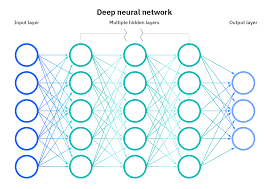
\includegraphics[width =7cm]{ProjectSubmissionFiles/download.png}
    \caption{Deep Neural Networks}
    \label{fig:my_label}
\end{figure}




% Acknowledgements should only appear in the accepted version.



\section{Convex Optimization of Neural Network:}
\subsection{Convex Neural Network}
Training multi-layer neural network involves infinitely many variables. Bengio et. al \cite{bengio2006convex} showed that this infinite variable problem can be converted to a convex optimization problem if the output loss function is convex in the neural network(NN) output and the output layer weights are regularized by a convex penalty. If precision limitations are imposed on all hidden units of a NN, a countable or even a finite set can be obtained. For such a NN, at the end what we get is an ordinary feedforward NN. This can be achieved by using a regularization penalty on the output weights that yield sparse solutions, such as the L1 penalty.
Let $x \in \mathbb{R}^d$ be the data matrix. $\bar x \in \mathbb{R}^{d+1}$ be an extension of the data matrix with one element 1. Let $h_i(x) = s(v_i.\bar x)$ where $s$ is the nonlinear activation function. Then the prediction is $\hat{y} = \sum_{i=1}^m w_ih_i(x)$. The goal is to learn $m$, $w_i'$s and $v_i$'s.\\
Let $\big{Q}$ be a convex regularization function and $\Omega(w) = \lambda \norm{w}_1$. Then the cost function becomes-
\begin{equation}
    C = \lambda \norm{w}_1 + \big{Q}(w.h(x_i), y_i)
\end{equation}
So, $Q$ and $\Delta$ is convex in $w$ and $C$ is a summation of both of them. So, $C$ is convex in $w$. 
NN can be seen as a convex optimization problem for infinite-dimensional space as long as the number of hidden units can be selected by the learning algorithm\cite{bengio2006convex}. have chosen a regularizer that generates a sparse solution to control the number of active hidden units and to transfer the problem into infinite dimensions. They have proved this in the case of hinge loss.\\
In terms of hinge loss, $\big{Q}(y,\hat{y}) = max(0, 1-y\hat{y})$. For this case the cost function is-
\begin{equation}
    C(w) = K\norm{w}_1 + \sum_{t=1}^n max(0, 1-y_tw.h(x_t))
\end{equation}

As constrained optimization problem, the cost function can be rewritten as the following-
\begin{equation}
    \begin{array}{l}
    \min_{\xi, w} K\norm{w}_1 + \sum_{t=1}^n \xi_t \\
    ~s.t.\quad y_t[w.h(x_t)] \geq 1-\xi_t \quad (C_1)\\
    \quad \xi_t \geq 0, ~for ~t = 1,2.....n \quad (C_2)
    \end{array}
\end{equation}
By taking the Lagrange multipliers of the constraints and the dual of this problem ($\max \sum_t q_th_i(x_t)$), according to \cite{hettich1993semi}, the solution of the dual can be attained with constraints $C_2$ and only $n + 1$ con- straints $C_1$. Their incremental ConvexNN algorithm is summarized in Algorithm- \ref{comvexnn}
\begin{algorithm}
\caption{ConvexNN}
   \label{comvexnn}
   %\SetAlgoLined
   \textbf{Input:} training set $D = {(x_1, y_1), . . . , (x_n, y_n)}$, convex loss function $Q$, and scalar regularization penalty $\lambda$. $s$ is either the sign function or the tanh function.
   \begin{algorithmic}[1]
      \STATE Set $v1 = (0, 0, . . . , 1)$ and select $w_1 = \min_{w_1} \sum_t Q(w_1s(1), y_t) + \lambda\norm{w_1}$
      \STATE i = 2
      \REPEAT
      \STATE Let $q_t = Q'(\sum{j=1}^{i-1} w_jh_j(x_t), y_t))$
      \IF{s = sign}{
        \STATE train linear classifier $h_i(x) = sign(v_i.\bar x)$ with examples ${(x_t, sign(q_t))}$ and errors weighted by $\mod{q_t}$, for $t = 1 . . . n $ (i.e maximize $\sum_t q_th_i(x_t)$)
      }
      \ELSIF{s = tanh}
        \STATE train linear classifier $h_i(x) = tanh(v_i.\bar x)$ to maximize $\sum_t q_th_i(x_t)$
    \ENDIF
    \UNTIL{$\sum_t q_th_i(x_t) \le \lambda$}
    \STATE Select $w_1, . . . , w_i$ (and optionally $v_2, . . . , v_i)$ minimizing $C = \lambda \norm{w}_1 + \big{Q}(w.h(x_i), y_i)$
    \STATE return the predictor $\hat{y_i} = \sum_j=1^iw_jh_j(x)$
   \end{algorithmic}
\end{algorithm}
They have proved that at termination the algorithm reaches global optima but it needs solving a sublinear problem involving a linear classifier with weighted errors. Another property of the algorithm is it behaves like boosting in the case of sign function when a linear classifier that minimizes the weighted cost is selected. In step 6, the algorithm requires to find the linear classifier. This is an NP-hard problem. They have mathematically proved that finding the linear classifier can be achieved in $\big{O}(n^3)$ steps when the input dimension is $2$. It can also be extended to multidimensional setting ($d$) where the complexity becomes $\big{O}(log(n)n^d)$. However, for higher dimensions, finding the exact minimizer is not a practical idea. Step 8 trains an approximation instead of an exact minimizer. Popular approximation techniques to find a linear classifier with the weighted cost is linear SVM, logistic regression, and the Perceptron algorithm. Considering the hinge loss doesn't generate a solution close to the exact minimum which is proved by their experimental results. In step 13, both $w$ and $v$ is optimized simultaneously. At the end of each stage, with a few training iterations of the whole NN using an ordinary gradient descent mechanism, one optimizes $w_j$’s and the $v_j$’s. Then $v_j$'s are fixed and $w_j$'s are optimized for that $v_j$'s. They have tested the algorithm with an exact and approximate linear classifier using a 2-d double moon toy dataset. The approximate algorithm has yielded an average test classification error of 3.68\% and the exact algorithm has yielded an average test classification error of 5.3\%.
\subsection{Global Convergence of Frank Wolfe on One Hidden Layer Networks }
Conditional gradients Frank-Wolfe algorithm is one of the well-known incremental algorithms for training one single hidden layer network. In a constrained minimization problem where projection on a set is hard, solving a Linear Minimization Oracle (LMO) is often easy using Frank Wolfe. Aspremont at. al \cite{d2020global} have shown that the LMO for one hidden layer NN can efficiently be solved under overparameterized and mild preconditioning assumptions. They have also shown that the overparameterized setting has a convex epigraph and no duality gap. They have focused on training the infinitely wide NN which is asymptotically convex. Like \cite{bengio2006convex} they have also considered a $L_1$ penalty to decide the locations of active neurons via the LMO. Each LMO adds a fixed number of neurons to the solution (In the case of \cite{bengio2006convex}, each iteration added a single neuron to the solution. 
1. The objective function can be written as follows-
\begin{equation}
\label{fweq}
    \begin{array}{l}
        minimize \sum _{i=1}^n (f(a_i) - y_i)^2 \\
        subject ~to\quad \gamma _1 (f) \leq \delta
    \end{array}
\end{equation}


Here $\gamma _1$is the variation norm(an extension to $L_1$ norm in infinite dimension). $A \in R^{n\times d}$ is the input data matrix, y is the output, and
\begin{equation}
    f(a_i) = \int \sigma _\theta (a_i)d\mu(\theta)
\end{equation}
Though equation \ref{fweq} is non-convex, for a large number of neurons and higher dimension, the objective becomes very close to convex. If started from one single unit, then the objective function becomes-
\begin{equation}
\begin{array}{cc}
     &  minimize \quad \norm{z-y}_2^2\\
     & subject~ to \quad \sigma(\theta^Ta_i) = z_i, ~ for~i=1,..,n
\end{array}
\end{equation}
Though this is non-convex, it's epigraph is convex when the number of neurons are greater than the number of sample. After taking the convex hull of its epigraph, the objective becomes-
\begin{equation}
\begin{array}{cc}
     &  minimize \quad \norm{z-y}_2^2\\
     & subject~ to \quad \sum_{j=1}^{n+2} \alpha_j\sigma(\theta_j^Ta_i) = z_i, ~ for~i=1,..,n
\end{array}
\end{equation}
So, in the case of training one single hidden layer network, the problem can be treated as convex when the number of neurons exceeds the sample size.
The activation function $\sigma_\theta$ is parameterized by $\theta \in \big{V}$ where $\big{V}$ is a compact topological vector space. $f(a_i) = \int \sigma _\theta (a_i)d\mu(\theta)$ is an action of the Radon measure $\mu$ on the activation function.
This is an infinite dimension problem that can be solved by Frank Wolfe where the LMO is solved over a $\gamma_1$ ball.
The Frank Wolfe invokes the LMO using the gradient at each iteration. Then the algorithm takes convex combinations of iterations. If the loss function if $L(f)$, then 
\begin{equation}
    L(f) = \sum _{i=1}^n (f(a_i) - y_i)^2 
\end{equation}
\begin{equation}
    L'(f) = \sum _{i=1} ^n g_i \delta 
\end{equation}
where,
\begin{equation}
    g_i = 2(\int \sigma _\theta (a_i)d\mu(\theta) - y_i)
\end{equation}
So the LMO that the Frank Wolfe solves becomes-
\begin{equation}
    minimize \sum_{i=1}^n g_if(a_i)
\end{equation}
By switching sums-
\begin{equation}
    \begin{split}
    &\inf_{\gamma_1( \int\sigma_\theta(·)d\mu(\theta)\leq 1} \sum_{i=1}^n g_i (\int \sigma _\theta (a_i)d\mu(\theta))\\
    &=  \inf_{\gamma_1( \int\sigma_\theta(·)d\mu(\theta)\leq 1}  (\int (\sum_{i=1}^n g_i\sigma _\theta (a_i))d\mu(\theta))\\
    & \geq -\max_{\theta \in \big{v}}\abs{\sum_{i=1}^n g_i\sigma _\theta (a_i)},
\end{split}
\end{equation}
if and only if $\mu = \mu_- - \mu_+$. So, the key of solving the LMO is solving $\max_{\theta \in \big{v}}\abs{\sum_{i=1}^n g_i\sigma _\theta (a_i)}$
The authors have solved this maximization problem for ReLU activation function. The overall algorithm is described in Algorithm \ref{fw}.
\begin{algorithm}[h]
\caption{Frank-Wolfe Algorithm}
\label{fw}
\textbf{Input:} A target precision $\epsilon > 0$
\begin{algorithmic}[1]
   \STATE Set $t := 1$, $\mu_1(\theta) = 0$.
   \REPEAT
   \STATE Get $\mu_d(\theta)$ solving (LMO) for $g_i$
   \STATE $g_i = 2(\int \sigma _\theta (a_i)d\mu_t(\theta) - y_i)$ for $i = 1,....n$
   \STATE Set $\mu_{t+1}_(\theta) := (1- \lambda_t)\mu_t(\theta) + \lambda_t\mu_d(\theta)$ for $\lambda := 2/(t+1)$
   \STATE Set t:= t+1
   \UNTIL{gap_t \leq \epsilon }\\
\end{algorithmic}
\textbf{Output:} $\mu(\theta)t_{max}$
\end{algorithm}
After T iterations, $L(\int \sigma _\theta ()d\mu_T(\theta)) - L^\star \leq \frac{4R^2\delta^2}{T+1}$ where $R^2 = \sup_{\theta \in \big{V}}\{\sum_{i=1}^n\sigma_\theta(a_i)^2\}$. Frank Wolfe also gives an upper bound of the duality gap $gap_t = \sum_{i=1}^ng_i(\int\sigma_\theta(a_i)d\mu_t(\theta) - \int\sigma_\theta(a_i)d\mu_d(\theta))$ where $\mu_t(\theta)$ is the current state and $\mu_d(\theta)$ is the solution of the linear minimization oracle.
When the number of sample $n$ is greater than the dimension $d$, the minimization objective becomes a finite sum problem. For this scenario, the authors have proposed a stochastic Frank Wolfe algorithm which solves a linear minimization oracle at each iteration on a subset of the samples. The sample size $m_t$ is equal to $(\frac{G(t+1)}{LD})^2$. Here $L$ is the Lipschitz constant and $G$ is the upper bound of the Lipschitz constant of the gradient of the objective function. For small $m_t$, the stochastic Frank Wolfe is similar to Algorithm \ref{fw}. The authors have tested the convergence of Frank Wolfe and Stochastic Frank Wolfe algorithms using toy examples. In the first case, the ground truth is generated using ten neurons in dimension 25 using Gaussian weights, observing 20 data points. In the case of Stochastic Frank Wolfe, the ground truth is generated by ten neurons, in dimension 20 using 25 samples. The empirical results show that overparameterized networks are inherently easier to train.
\subsection{Convex Relaxation for shallow neural networks }
In this paper, the neural network model the author considers is shallow network, which only contains one hidden layer.it is much easier to analyze. Also, with the number of neurons increases, shallow neural network can approximate any functions,which has important practical significance. In the following part, the derivation of convex relaxation will be shown from the simplest case (i.e. one neuron in hidden layers) to multiple neuron case. The author shows such generalization is always held. \\
For single neuron case, assume there exists planted parameter $x^*$, the model considered here is:
\begin{equation}
    y=g(Ax^*)
\end{equation}
the objective function is:
\begin{equation}
    \min_{x}\frac{1}{2}f(x)=\min_{x}\frac{1}{2}\left \| g(Ax)-y \right \|_2^2
\end{equation}
Where $g(.)$ is the ReLU activation function: $g(x)=max(0,x)$, $A\in R^{n\times d}$ is the input data matrix, $x\in R^d$ is the parameter vector for first layer and y is considered from the planted model such that $y=g(Ax^*)$\\
Taking gradient of $f(x)$:
\begin{equation}
    \triangledown f(x)=A^TD(g(Ax_t)-y)
\end{equation}
Where $D_t$ is the diagonal matrix and its $i^{th}$ diagonal entry is computed as 1 if $a_i^T x\geq 0$, 0 otherwise. \\
The objective above function may not be a convex function because of the existence of ReLU.However, if we expand Objective function $f(x)$ and relax it as:
\begin{equation}
    f_r(x)=\left \| g(Ax) \right \|_2^2-2y^TAx+\left \| y \right \|_2^2
\end{equation}
The author shows that $f_r(x)$ is convex (Proposition 1.) and also holds the same optimal value as $f(x)$. (Theorem 1.)\cite{cvxrelxation}. Thus, by convex function property, $f_r(x)$ will only have one global minimum. Gradient descent with proper step size will converge to the global minimum.\\
When it comes to the hidden layer with multiple neurons, instead of considering the model $y=g(Ax^*)$, the model is:
\begin{equation}
    y_i=\sum_{1}^{m}g(a_i^Tx_j^*) \forall{i\in 1....n}
\end{equation}
$x_j^*$ is the planted parameter vector of each neuron. Similarly as single neuron case, the objective function is defined as:
\begin{equation}
    \min_Xf_m(X)=\min_X \frac{1}{2}\left \| \sum_{j=1}^{m}g(Ax_j)-y \right \|_2^2
\end{equation}
Where $g(.)$ is still the ReLU activation function, $A\in R^{n\timesd}$ is input matrix.\\
The objective function has multiple global minimum points, because if we permute $x_j$ from different orders, they are all global optimum solutions. If $n > d$,we can obtain more equations than true parameters, thus, gradient descent still works in this case. If $n \leq d$, in this case, we cannot compute all the true parameters. Gradient descent may fail to converge to the global optimum. Thus, the importance of convex relaxation will show up.\\
If we denote the residual as $r=\sum_{j=1}^{m}g(Ax_j)-y$, the gradient can be denoted as:
\begin{equation}
    \triangledown {x_j} f_m(X)=2A^TD_jr
\end{equation}
Apply first-order condition (i.e $\triangledown {x_j} f_m(X)=2A^TD_jr=0\ \forall j=1..m$), if A is assumed to be full rank, then the optimal condition is achieved if and only if $D_jr=0\ \forall j=1..m$. However, $D_j$ is a low rank diagonal matrix, if the corresponding element is 0, then the corresponding index in r can be arbitrary number, which indicates gradient descent may fail to converge to the optimal value.\\
In order to overcome the problem taken by the low rankness of $D_j$, the modified gradient descent algorithm is:
\begin{equation}
    \triangledown {x_j} f_m(X)=2A^TD_jr+2A^T\prod_{j=1}^{m}D_j^cr
\end{equation}
Where $D_j^c=I_n-D_j$. With this modification, we can guarantee that each index of residual has a positive multiplicative factor so that $\triangledown_{x_j} f_m(X)=0$ implies $r=0$.\\
The corresponding function satisfies the modified gradient is:
\begin{equation}
    f_{mp}(X)=\left \| \sum_{j=1}^{m}g(Ax_j)-y \right \|_2^2-2y^T\prod_{j=1}^{m}D^c_jA\sum_{j=1}^{m}x_j
\end{equation}
It is proved that the relaxation of original objective function is convex \cite{cvxrelxation} and it preserve the same optimal value as the original objective function $f_m$. Thus, applying gradient descent with proper step size, it can guarantee modified gradient descent converge to the unique optimal value. 
\subsubsection{Numerical Experiments}
The author generates the input and output data and initialize the parameter vector/matrix according to standard normal distribution. Then, the author uses shallow network with single neuron and multiple neurons to show the training and test performance,which are in Figure 1 and Figure 2 \cite{cvxrelxation}.When the number of sample (n) is larger than d, during training process, both objective value of original function and relaxed function will achieve to 0, which confirms the property that convex relaxation doesn't change the optimal value. When n is smaller than or equal to d, it indicates the regularized gradient descent converges faster than gradient descent algorithm. It possibly confirms the reason why gradient descent may fail even in shallow network with non-convex objective function. However, this convex relaxation only applies to shallow network, which is quite limited. Further research can be done to test whether we can achieve such convex relaxation on Deep ReLU network.
\subsection{Revealing the Structure of Deep Neural Networks via Convex Duality }
This paper mainly uses the existing convexity of dual problem for objective function and uses the extreme point condition in constraint to compute the explicit solution of each layer weight matrix of neural networks. As a result, the strong duality holds for regularized training problem and its weight coincides with the iterative methods such as SGD.
Recall the general optimization problem:
\begin{equation}
    \begin{array}{rrclcl}
    \displaystyle \min_{x} & \multicolumn{3}{l}{f_0(x)}\\
    \textrm{s.t.} &f_i(x)\leq 0\\
    &h_i(x)=0    
\end{array}
\end{equation}
The lagrangian function is defined as:
\begin{equation}
    L(x,\lambda,\nu)=f(x)+\sum_{i=1}^{m}\lambda_if_i(x)+\sum_{i=1}^{p}\nu_i h_i(x)
\end{equation}
And the dual problem is $D^*=\max \inf L(x,\lambda,\nu)$. No matter whether f(x) is convex or not, the $\inf L(x,\lambda,\nu)$ is a concave function. Thus, maximize a concave function is a convex optimization problem. \cite{boydcvx}. This is why idea how to connect duality with convexity and apply them into neural network training problem. 

\subsubsection{two-layer linear network}
In order to give a more precise explanation for how to use duality to compute the weight matrix of neural network. The minimum norm variant problem is first considered as the following:
\begin{equation}
    \min_{\theta \in \Theta } \left \| W_1 \right \|_F^2+\left \| w_2 \right \|_2^2 \ \ s.t. \ \ f_{\theta,2}(X)=y
\end{equation}
Where $W_1 \in R^{d\times m}$ is the weight matrix connecting input layer and hidden layer, $w_2\in R^m$ is the weight vector connecting hidden layer and output layer. $X\in R^{n\times d}$ is the input matrix and $y\in R^n$ is the output respectively. By Lemma A.1 \cite{cvxduality1}, it is equivalent as:
\begin{equation}
    P^*=\min_{\theta \in \Theta}\left \| w_2 \right \|_1 \ \ s.t \ \ f_{\theta,2}(X)=y,\ \ w_{1,j}\in B_2,\forall j 
\end{equation}
Using duality scenario, the dual problem (with strong duality holds) is given by:
\begin{equation}
    \begin{split}
    \centering
        &P^*=D^*\\
        &=\max_\lambda \lambda^Ty \ \ s.t. \ \ \left \| (XW_1)^T\lambda \right \| \leq 1\ \ \forall \left \|w_{1,j}\right \|_2^2\leq 1\forall j \\
        &=\max_{\lambda \in R^n} \lambda^Ty \ \ s.t. \ \ \max_{w_1 \in B_2} \left | \lambda^TXw_1 \right | \leq 1
    \end{split}
\end{equation}
Here $B_2$ is the unit ball constraint with squared norm (i.e $\left \| u \right \|_2 \leq 1$.The optimal solution is obtained on the boundary of the constraint $\max_{w_1\in B_2} \left |  \lambda^*^TXw_1\right |\leq 1$.\\
Assume that there exists a planted parameter $w^*$ such that $X w^*=y$ holds, then apply Singluar Value Decomposition(SVD) on original input matrix X, the problem can be reformulated as:
\begin{equation}
    \begin{aligned}
    \max_{\widetilde{\lambda}} \quad & \widetilde{\lambda} \Sigma _x \widetilde{w}^*\\
    \textrm{s.t.} \quad & \left \| \Sigma_x\widetilde{\lambda} \right \|_2 \leq 1 \\
    \end{aligned}
\end{equation}
Where $\widetilde{\lambda}=U_x^T\lambda$ and $\widetilde{w^*}=V_x^T w^*$. When $\Sigma_x^T\widetilde{\lambda}=c_1\widetilde{w}^*$, the optimal neuron (i.e, each column of $W_1$) should satisfy the following condition:
\begin{equation}
    w_1^*=\frac{V_x\Sigma_x \widetilde{\lambda}}{\left \| V_x \Sigma_x\widetilde{\lambda} \right \|_2}=\frac{V_x\widetilde{w}_r^*}{\left \| \widetilde{w}_r^* \right \|_2}=\frac{P_{X^T}(w^*)}{\left \| P_{X^T}(w^*) \right \|_2}
\end{equation}
The above scenario can be summarized as: first, derive the dual problem, which has strong duality property and it is also a standard convex optimization problem; second, the optimal solution should be the extreme points of the constraint.\\
Following this scenario, the primal and dual regularized training problem for two-layer linear network are:
\begin{equation}
    \begin{aligned}
    &P^*=\min_{\theta \in \Theta} \left \|f_{\theta,2}(X)-y\right \|_2^2+\beta\left \| w_2 \right \|_2^2 \ \ s.t.\ \ w_{1,j}\in B_2\\
    &D^*=-\frac{1}{2}\left \| \lambda-y \right \|_2^2+\frac{1}{2}\left \| y \right \|_2^2 \ \ s.t. \ \ \max_{w_1 \in B_2}\left | \lambda^TXw_1 \right |\leq \beta
    \end{aligned}
\end{equation}
Strong duality also holds in this case(Theorem 2.2 \cite{cvxduality1}. Solving above dual objective function by optimal condition ($\lambda=y$) and plug it into the constraint to satisfy the extreme point condition, the explicit for $w_1$ is:
\begin{equation}
    w_1^*=\frac{X^TP_{X,\beta}(y)}{\left \|X^TP_{X,\beta}(y)\right \|_2^2}
\end{equation}
Where $P_{X,\beta}$ projects to $\left \{ u\in R^n | \left \| X^Tu \right \|_2 \leq \beta \right \}$
\subsubsection{two-layer linear network with vector outputs}
Unlike the weight vector $w_2$ for previous problem, in this case, $W_2 \in R^{m\times n}$ will become a matrix satisfying $f_{\theta,2}(X)=XW_1W_2$, $Y\in R^{n\times K}$, the primal and dual of the minimum norm variant problem is:
\begin{equation}
    \begin{aligned}
        &P^*=\min_{\theta \in Theta} \left \| W_1 \right \|_F^2+\left \| W_2 \right \|_F^2\ \ s.t. \ \ f_{\theta,2}(X)=Y\\
        &=\min_{\theta \in Theta}\sum_{j=1}^{m}\left \| w_{2,j} \right \|_2 \ \ s.t. \ \ f_{\theta,2}(X)=Y,\ \ w_{1,j} \in B_2\\
        &D^*= \max_{\Lambda }tr(\Lambda Y)\ \ s.t\ \  \left \| \Lambda^TXw_1 \right \|_2 \leq 1, \forall w_1 \in B_2
    \end{aligned}
\end{equation}
Strong duality holds for above equation(Theorem 2.3\cite{cvxduality1}).Suppose there exists a planted parameter $W^*$ such that $Y=XW^*$,The solution for optimal neuron is still the extreme points of constraint$\left \| \Lambda^TXw_1 \right \|_2 \leq 1, \forall w_1 \in B_2$, which is the subset of first $rank(W^*)$ largest right singular vectors of $\Lambda^TX$.\\
Similarly, for the regularized training problem with vector output, the primal and dual problem is:
\begin{equation}
    \begin{aligned}
        &P^*=\min_{\theta \in \Theta}\frac{1}{2}\left \| f_{\theta,2}(X)-Y \right \|_F^2+\beta \sum_{j=1}^{m}\left \| w_{2,j} \right \|_2 \ \ s.t w_{1,j} \in B_2 \\
        &D^*=\max_{\Lambda} -\frac{1}{2}\left \| \Lambda-Y \right \|_F^2+\frac{1}{2}\left \| Y \right \|_F^2 \ \ s.t \sigma_{max}(\Lambda^TX)\leq \beta\\
    \end{aligned}
\end{equation}
Strong duality holds for above problems(Theorem 2.4 \cite{cvxduality1}).The optimal solutions for dual problem is the subset of maximal right singular vectors of $P_{X,\beta}(Y^T)X$, where $P_{X,\beta}(.)$ projects vector into the set $\left \{ U \in R^{n\times K} | \sigma_{max}(U^TX) \leq \beta \right \}$.
\subsubsection{Deep Linear Networks}
Unlike the usual expression for deep linear networks (i.e $f_{\theta,L}=XW_1 W_2 ... \mathbf{w_{L-1}}w_L$, the layer weight matrix is setting as: $f_{\theta,L}=\sum_{j=1}^{m} XW_{1,j}...w_{L,j}$,then for the training problem:
\begin{equation}
    \min_{\left \{ \theta_l \right \}_1^L} \frac{1}{2}\sum_{j=1}^{m}\sum_{l=1}^{L}\left \| W_{l,j} \right \|_F^2\ \ s.t. \ \ f_{\theta,L}=y
\end{equation}
\begin{theorem}
    Optimal layer weights for (33) is:\\
    $W_{l,j}^*=\left\{\begin{matrix}
    t_j^*\frac{V_x\widetilde{w}^* }{ \left \| \widetilde{w_r}^* \right \|_2 }\rho_{1,j}^T, \ \ l=1\\ 
    t_j^* \rho_{l-1,j}\rho_{l,j}^T,\ \  1<l\leq L-2\\ 
    \rho_{L-2,j}, \ \ l=L-1
    \end{matrix}\right.$
\end{theorem}
Where $\rho_{l,j}\ \in\ \ R^{m_l}$ such that $\left \| \rho_{l,j} \right \|_2=1 \ \ \left \langle \rho_{l,j},\rho_{l,k} \right \rangle=0 \ \ \forall l \in \left \{1....L-2  \right \} \ \ \forall j,k \in \left \{1....m  \right \}$. $w_r^*$ preserve the first r element and the rest equals to 0, where r is the rank of X.Besides, the strong duality also holds for dual of (34). \\
However, if plugging first layer weight, we can find:$XW_1\rho1=cy$ holds. Thus, the rest layer actually contributes nothing to the expressive power of the network.\\
Similarly, for regularized training problem:
\begin{equation}
    \min_{\left \{ \theta \right \}_1^L}\frac{1}{2}\left \| f_{\theta,L}(X)-y \right \|_2^2 +\frac{\beta}{2}\sum_{j=1}^{m}\sum_{l=1}^{L}\left \|  W_{l,j}\right \|_F^2
\end{equation}
\begin{theorem}
    Optimal layer weights for (34) is:\\
    $W_{l,j}^*=$
    \begin{cases}
    t_j^*\frac{X^TP_{X,\beta}(y) }{ \left \| X^TP_{X,\beta}(y) \right \|_2 }\rho_{1,j}^T, \ \  l=1\\ 
    t_j^* \rho_{l-1,j}\rho_{l,j}^T,\ \ 1<l\leq L-2\\ 
    \rho_{L-2,j}, \ \ l=L-1
    \end{cases}
\end{theorem}
Where $P_{X,\beta}$ projects to the set $\left \{ u \in R^n|\left \| X^Tu \right \|_2 \leq \beta t_j^{*2-L} \right \}$. Strong duality also holds for (35) \cite{cvxduality1}.
\subsubsection{Deep Linear network with vector output }
In this case, the L-layer deep linear network model should be described as:$f_{\theta,L}(X)=\sum_{j=1}^{m}XW_{1,j}....\mathbf{w_{L,j}^T}$.\\
Strong duality also holds in this case and the optimal neuron can be computed explicitly similarly as deep linear network with scalar output. The key difference in expression is the first layer weight matrix. For regularized training problem, instead using $\frac{X^TP_{X,\beta}(y) }{ \left \| X^TP_{X,\beta}(y) \right \|_2 }$, we need to compute the maximal right singular vector of $P_{X,\beta}(Y)^TX$, which is extremely similar as the analysis for two-layer linear network with vector output. 
\subsubsection{Deep ReLU Networks}
Here, we consider a L-layer ReLU network with the output function $f_{\theta,L}(X)=A_{L-1}w_L$, where $A_{l,j}=(A_{l-1,j}W_{l,j})_+, A_{0,j}=X, \ \ \forall l,j $\ \ and $(x)_+=max(0,x)$ (definition of ReLU).
The minimum norm variant problem can be formulated as:
\begin{equation}
    \min_{\left \{ \theta_l \right \}_1^L}\sum_{j=1}^{m}\sum_{l=1}^{L}\left \| W_{l,j} \right \|_F^2 \ \ s.t \ \ f_{\theta,L}(X)=y
\end{equation}
\begin{theorem}
    Let X be rank-one matrix such that $X=\mathbf{c}\mathbf{a_0^T}$, where $\mathbf{c}\in R^n_+$ and $\math{a_0} \in R^d$, then strong duality holds and optimal weights are:\\
    $W_{l,j}=\frac{\phi _{l-1,j}}{\left \| \phi_{l-1,j} \right \|} \phi _{l,j}^T, \ \ \forall l\in [L-2], \ \ w_{L-1,j}=\frac{\phi_{L-2,j}}{\left \| \phi_{L-2,j} \right \|_2}$\\
    where $\phi_{0,j}=a_0$ and $\left \{ \phi_{l,j} \right \}_{l=1}^{L-2} $ a set of vectors such that $\phi_{l,j}\in R_+^{m_l}$ and $\left \|\phi_{l,j}  \right \|_2=t_j^*$
\end{theorem}

\subsubsection{Regularized problem with vector output}
Now, the last layer has multiple neurons thus the shape of output matrix $Y\in R^{n\times K}$. if we focus on the minimum norm variant problem, the results stated in last theorem still holds for vector output case. However, from above results, when the model has L layers, we can only compute L-1 layers explicitly. \\
In order to compute the full layer weights explicitly, additional assumptions are needed:
\begin{theorem}
    Let $\left \{X,Y \right \}$ be a dataset such that $XX^T=I_n$ and Y is one-hot encoded, then a set of optimal solutions for the following regularization training problem:
    \begin{equation}
        \min_{\theta \in \Theta}\frac{1}{2}\left \| f_{\theta,L}(X)-Y \right \|_F^2+\frac{\beta}{2}\sum_{j=1}^{m}\sum_{l=1}^{L}\left \| W_{l,j} \right \|_F^2
    \end{equation}
    can be formulated as:\\
    $W_{l,j}=\begin{cases}
    \frac{\phi_{l-1,j}}{\left \| \phi_{l-1,j} \right \|_2} \phi^T_{l,j} , \ \ if \ \ l\in [L-1]\\
    \left ( \left \| \phi_{0,j} \right \|_2-\beta \right )_+ \phi_{l-1,j}e^T_r, \ \ if \ \ l=L
    \end{cases}$ \\
    where $\phi_{0,j}=X^Ty_j$, $\left \{ \phi_{l,j} \right \}_{l=1}^{L-2}$ is set of vectors such that $\phi_{l,j} \in R^{m_l}_+, \left \| \phi_{l,j}=t_j^* \right \| $ and $\phi_{l,i}^T\phi_{l,j}=0, \ \ \forall i \neq j$, Moreover, $\phi_{L-1,j}=e_j$ is the $j^{th}$ ordinary basis vector. 
\end{theorem}
Strong duality also holds for optimization problem (37).
\subsubsection{Numerical Experiments and Conclusion}
During the mathematical deduction, there are some interesting properties which are not covered in previous part. The first is for deep linear network, the rank of first (L-1) layer weight matrix is dependent on $\beta$. The second is for deep linear network, the Frobenius norm of first (L-2) layers is the same.At first, the author uses the data generated from standard normal distribution to verify above claims and also test the strong duality property. Then, the author use real dataset CIFAR-10 \cite{CIFAR} and MINIST to test the computed parameter with layer L=3,4,5. From Figure 4\cite{cvxduality1}, as the epoch increases, the training and test error computed by SGD will finally converge to the result computed by convex duality, which proves the result in theory part. However, this paper has strict assumptions for input data and output data when the structure comes into deep ReLU case, which is not practical in reality. It still needs to be expanded into more general assumptions.
\subsection{Global Optimality Beyond Two layers: Training Deep ReLU Networks via Convex Programs }
In this paper, the idea for "Convex Program" is still from the convexity in duality. However, unlike deep linear network or deep ReLU network considered in the last paper. In this paper, the neural network structure consists of K L-layer sub-networks. In particular, 3-layer structure is used in sub-network structure for deduction(Figure2).
\begin{figure}[H]
    \centering
    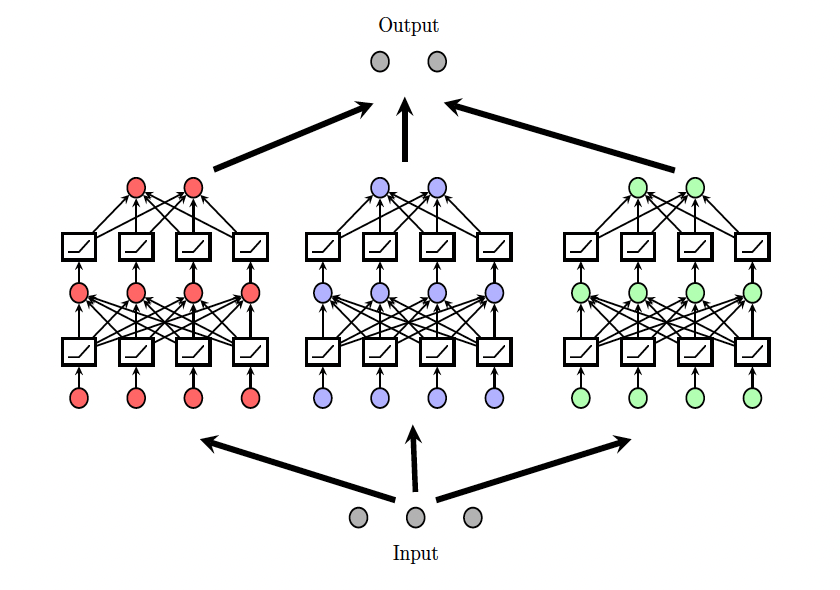
\includegraphics[scale=0.4]{ProjectSubmissionFiles/Fig1.png}
    \caption{Architecture of sub-networks }
    \label{fig1}
\end{figure}
In this article, the author uses $X\in R^{n\times d}$ to denote the input matrix. $\theta=\left \{ \left \{ W_{lk} \right \}_{l=1}^L \right \}_{k=1}^K $, where l represents the $l^{th}$ layer in sub-network, k represents the $k^{th}$ sub-network respectively. $W_{lk}$ is the weight matrix of layer $l$ in $k^{th}$ sub-network. \\ 
A natural question arises why this type of structure is important. Consider the structure of Residual block (Figure 2 in \cite{Resnet}), its structure can be characterized in sub-network form:$W_{11}=W_1$, $W_{21}=W_2$, $W_{12}=W_{22}=I$, $W_{31}=W_{32}=w_3$. Thus, once the results of training deep ReLU networks can be achieved by convex optimization, it has important applications in many neural network structures.\\
Given dataset $\left \{\mathbf{X},\mathbf{y}  \right \}$ with $L=3$, the regularized training problem can be formulated as:
\begin{equation}
    P^*=\min_{\theta \in \Theta}\frac{1}{2}\left \| f_\theta(X)-y \right \|_2^2+\frac{\beta}{2}\sum_{k=1}^{K}(\left \| w_{2k} \right \|_2^2+w_{3k}^2)
\end{equation}
Where $\Theta=\left \{ \theta: \left \| W_{1k} \right \|_F \leq 1\ \ \forall k \in [K]\right \}$ and $f_{\theta}(X)=\sum_{k=1}^{K}f_{\theta,k}(X) $. The above problem is equivalent as:
\begin{equation}
    P^*=\min_{\theta \in \Theta_p} \frac{1}{2} \left \| f_\theta(X)-y \right \|_2^2+\beta\left \| w_3 \right \|_1
\end{equation}
Where $\theta_p=\left \{ \theta: \left \| W_{1k} \right \|_F \leq 1,\left \| W_{2k} \right \|_F\leq 1, \forall k \in [K]\right \}$.\\
Take the dual with respect to $w_3$ and change the order of min-max to obtain the dual problem:
\begin{equation}
    \begin{aligned}
        &P^* \geq D^*=\max_{v}-\frac{1}{2} \left \| v-y \right \|_2^2+\frac{1}{2} \left \| y \right \|_2^2 \\
        &s.t\ \  \max_{\theta \in \Theta_p} \left | v^T((XW_1)_+w2)_+ \right | \leq \beta
    \end{aligned}
\end{equation}
Where $(.)_+$ is the representation of ReLU activation. Then, we also derive the bidual of (39), that is, taking dual form with respect to v in (40), the bidual can be formulated as:
\begin{equation}
    \begin{aligned}
        &P^*_B= \min_{\mu}\frac{1}{2}\left \| \int _{\theta \in \Theta_p}((XW_1)_+w_2)_+  \right \| _2^2+ \beta \left \| \mu \right \|_{TV} \\
        &=\min_{\theta \in \Theta_p} \frac{1}{2} \left \| \sum_{i=1}^{K^*}f_{\theta, i}(X)-y\right \|_2^2+\beta \left \| w_3 \right \|_1.
    \end{aligned}
\end{equation}
The above equivalence can be shown by Caratheodory's theorem. And \cite{deeprelu} shows that strong duality holds for $P_B^*=D^*$. Because (41) is the same as (39) with $K^* \geq K$. Thus, strong duality also holds $P^*_B=P^*=D^*$. However, due to the existing of ReLU function in constraint of $D^*$, this problem cannot be solved by standard convex optimization solver directly. It needs to be represented into a standard convex constraint. Following the results in the paper\cite{deeprelu}, the constraint $ \max_{\theta \in \Theta_p}\left | v^T((XW_1)_+w_2)_+ \right | \leq \beta$ is equivalent as :
\begin{figure}[H]
    \centering
    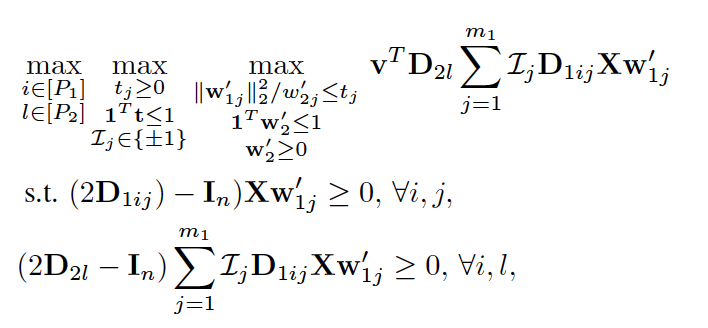
\includegraphics[scale=0.6]{ProjectSubmissionFiles/Fig2.png}
\end{figure}
Where $D_{1ij} \in R^{n\times n}$ and $D_{2l} \in R^{ n\times n}$ are the sequence of diagonal mask matrix, which aims to simulate the behavior of ReLU. If the value after ReLU activation is still itself, then the corresponding diagonal value of $D_{1ij}$ or $D_{2l}$ is 1, otherwise it is 0.(see \cite{deeprelu} for details, the deduction for notation is omitted here.) $w'_{1j}=\sqrt{w'_{2j}}w_{1j}$ and $w'_{2j}=w_{2j}^2$, they are all the $j^{th}$ column of $W_1$ and $W_2$ respectively. Use this constraint, the derived bidual form $P_B^*$ can be formulated as:
\begin{theorem}
    The non-convex training problem (38) can be equivalent stated as a convex problem as follows:\\
    \begin{equation}
            \min_{w,w' \in C}\frac{1}{2}\left \| \widetilde{X}(w'-w)-y \right \|_2^2+\beta(\left \| w \right \|_{2,1}+\left \| w' \right \|_{2,1})
    \end{equation}
    where $\left \| . \right \|$ is a dimensional group norm operator such that given a vector $u\in R^{dp}$, $\left \|  u\right \|_{2,1}=\sum_{i=1}^{P}\left \| u_i \right \|_2$, where $u_i$'s are ordered d dimensional partitions of u. Moreover, $\widetilde{X} \in R^{n\times 2dm_1P_1P_2}$ and C are defined as:
    \begin{figure}[H]
        \centering
        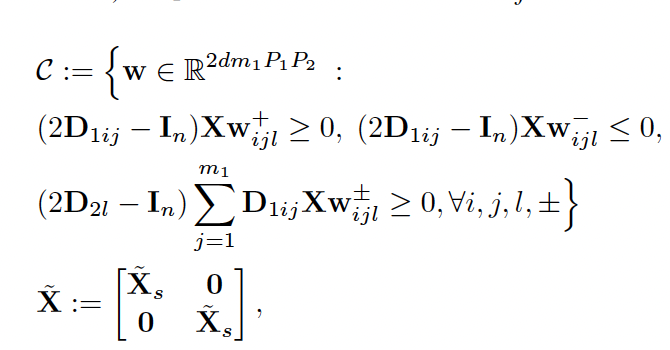
\includegraphics[scale=0.7]{Fig3}
    \end{figure}
    where $w,w'\in R^{2dm_1P_1P_2}$ are the vectors constructed by concatenating $\left \{ \left \{ \left \{ \left \{ w_{ijl}^{\pm} \right \}_{i=1}^{P_1} \right \}_{j=1}^{m_1} \right \}_{l2=1}^{P_2} \right \}_{\pm}$ and $\left \{ \left \{ \left \{ \left \{ w'_{ijl}^{\pm} \right \}_{i=1}^{P_1} \right \}_{j=1}^{m_1} \right \}_{l2=1}^{P_2} \right \}_{\pm}$ respectively, and\\
    $\widetilde{X}_s=\left [ D_{21}D_{111}X...D_{2l}D_{1ij}X...D_{2P_2}D_{1P_1m_1}X \right ]$
\end{theorem}
In order to solve the problem stated in Theorem 5. We need first to simulate the series of $\left \{\left \{ D_{1ij} \right \}_{i=1}^{P_1} \right \}_{j=1}^{m_1}$ and $\left\{D_{2l}\right\}_{l=1}^{P_2}$, where $P_1$ is the number of positive sign after $(Xw),\for w\in R^d$($w$ is the connecting layer between input data and first layer of sub-networks), $P_2$ is the number of positive sign after $((X W_1)_+w_2)$.They are all in polynomial time complexity with respect to input dimension $n$ and $d$ \cite{deeprelu}. \\
To achieve simulation, generate $\mathbf{u_{ij}}$ from $N(0,\mathbf{I_d})$ for $P_1$ times and let $D_{ijl}=diag(\textbf{1}[\mathbf{Xu_{ij}}\geq 0)$. Similarly, generate $\mathbf{U_1}\in R^{d\times m_1}$ and $\mathbf{u_2} \in R^{m_1} P_2$ times and set $D_{2l}=diag(\textbf{1}[(\mathbf{XU_{1l})_+u_{2l}}]\geq 0)$, Then, use the standard solver CVX to solve this problem. According to the complexity of interior point methods, the paper \cite{deeprelu} also proves that this problem can be trained in polynomial time with respect to $n$ and $d$,which indicates this problem is a practical problem for computing. \\
After introducing the formulation of the solution, from the series of diagonal matrix, it leads us to rethink about the role of ReLU.For this subnetwork, it has two ReLU-layer, which can be interpreted as a high-dimensional feature selection method due to convex group sparsity regularization \cite{deeprelu}.Thus, this results reveals the impact of having additional layers and its implication on the expressive power of a network. \\
\subsubsection{Numerical Experiment}
The author first conducts experiment to verify the strong duality holds between (38) and (42). Input data matrix X is generated by standard Gaussian distribution with (n,d)=(5,2). The 3-layer sub-network has structure $m_1=3$ and $K=2,5,15$.Then, the author uses SGD to train (38) and use convex program to train (42). It is found that when K is small, the SGD may be easily get stuck in local minimum. However, with K increases, this phenomena will disappear, SGD will converge to the optimal value, which is same as the optimal value obtained by convex program. The result is shown in Figure 4 \cite{deeprelu}\\
At last, the author conduct experiment on CIFAR-10\cite{CIFAR} and Fashion-MNIST dataset \cite{xiao2017/online}. The sub-network structure is $L=3$, $m_1=100$,$K=40$. The result is shown in Figure 5 \cite{deeprelu}.
It is shown that the accuracy obtained by convex program is higher than SGD training. For details,please see Figure 5 in \cite{deeprelu}. 
% In the unusual situation where you want a paper to appear in the
% references without citing it in the main text, use \nocite

\section{Conclusion}
The goal of this literature is to discover different existing techniques of convex optimization of neural network. Optimization of infinitely wide neural networks is asymptotically convex. The first two papers apply L-1 regularization to make this infinite variable problem finite. Convex neural network solves an exact or approximate linear classifier at each step. Global convergence bound can be achieved for L1 regularized neural network using Frank Wolfe algorithm.The third paper utilize one global minimum property of convex function, which eliminate the possible failure of gradient descent in non-convex setting. The fourth and fifth paper utilize the convexity in dual problem and transform the original non-convex problem into a convex problem, which is practical in time complexity and also applicable because of its better performance. There are also many interesting convex problems in Neural Network training that don't contain in this literature review. For example, one can use convex optimization to compute the sparse representation of original weight matrix, which will improve the efficiency of training a neural network, using dual convexity to describe the mechanism of back-propagation. Further combination of convex optimization and neural network may be focused more on generalizing these results into more complicated neural network structures with less restrictive assumptions. Hopefully, with the assistance of convex optimization, training neural network will not be a "black-box" problem soon.

\nocite{langley00}

\bibliography{bib_tex}
\bibliographystyle{icml2021}


%%%%%%%%%%%%%%%%%%%%%%%%%%%%%%%%%%%%%%%%%%%%%%%%%%%%%%%%%%%%%%%%%%%%%%%%%%%%%%%
%%%%%%%%%%%%%%%%%%%%%%%%%%%%%%%%%%%%%%%%%%%%%%%%%%%%%%%%%%%%%%%%%%%%%%%%%%%%%%%
% DELETE THIS PART. DO NOT PLACE CONTENT AFTER THE REFERENCES!
%%%%%%%%%%%%%%%%%%%%%%%%%%%%%%%%%%%%%%%%%%%%%%%%%%%%%%%%%%%%%%%%%%%%%%%%%%%%%%%
%%%%%%%%%%%%%%%%%%%%%%%%%%%%%%%%%%%%%%%%%%%%%%%%%%%%%%%%%%%%%%%%%%%%%%%%%%%%%%%

%%%%%%%%%%%%%%%%%%%%%%%%%%%%%%%%%%%%%%%%%%%%%%%%%%%%%%%%%%%%%%%%%%%%%%%%%%%%%%%
%%%%%%%%%%%%%%%%%%%%%%%%%%%%%%%%%%%%%%%%%%%%%%%%%%%%%%%%%%%%%%%%%%%%%%%%%%%%%%%


\end{document}


% This document was modified from the file originally made available by
% Pat Langley and Andrea Danyluk for ICML-2K. This version was created
% by Iain Murray in 2018, and modified by Alexandre Bouchard in
% 2019 and 2021. Previous contributors include Dan Roy, Lise Getoor and Tobias
% Scheffer, which was slightly modified from the 2010 version by
% Thorsten Joachims & Johannes Fuernkranz, slightly modified from the
% 2009 version by Kiri Wagstaff and Sam Roweis's 2008 version, which is
% slightly modified from Prasad Tadepalli's 2007 version which is a
% lightly changed version of the previous year's version by Andrew
% Moore, which was in turn edited from those of Kristian Kersting and
% Codrina Lauth. Alex Smola contributed to the algorithmic style files.
